\subsection{Sinusoid regression with MAML}

Following the connections between MAML and hierarchical Bayes explored by \citet{grant2018recasting}, we also explored regression on sinusoids using MAML. Our aim was to investigate how predictive our linear theory is for this highly non-linear problem setting. As in \citet{finn2017model}, we sample sinusoid functions by placing a prior over the amplitude and phase. In other works \citep{finn2017model, grant2018recasting} the same prior is used for the training and testing stages. However, to better measure generalization to novel tasks we use different prior distributions when training versus evaluating the model.

\iflatexml
\begin{figure}
    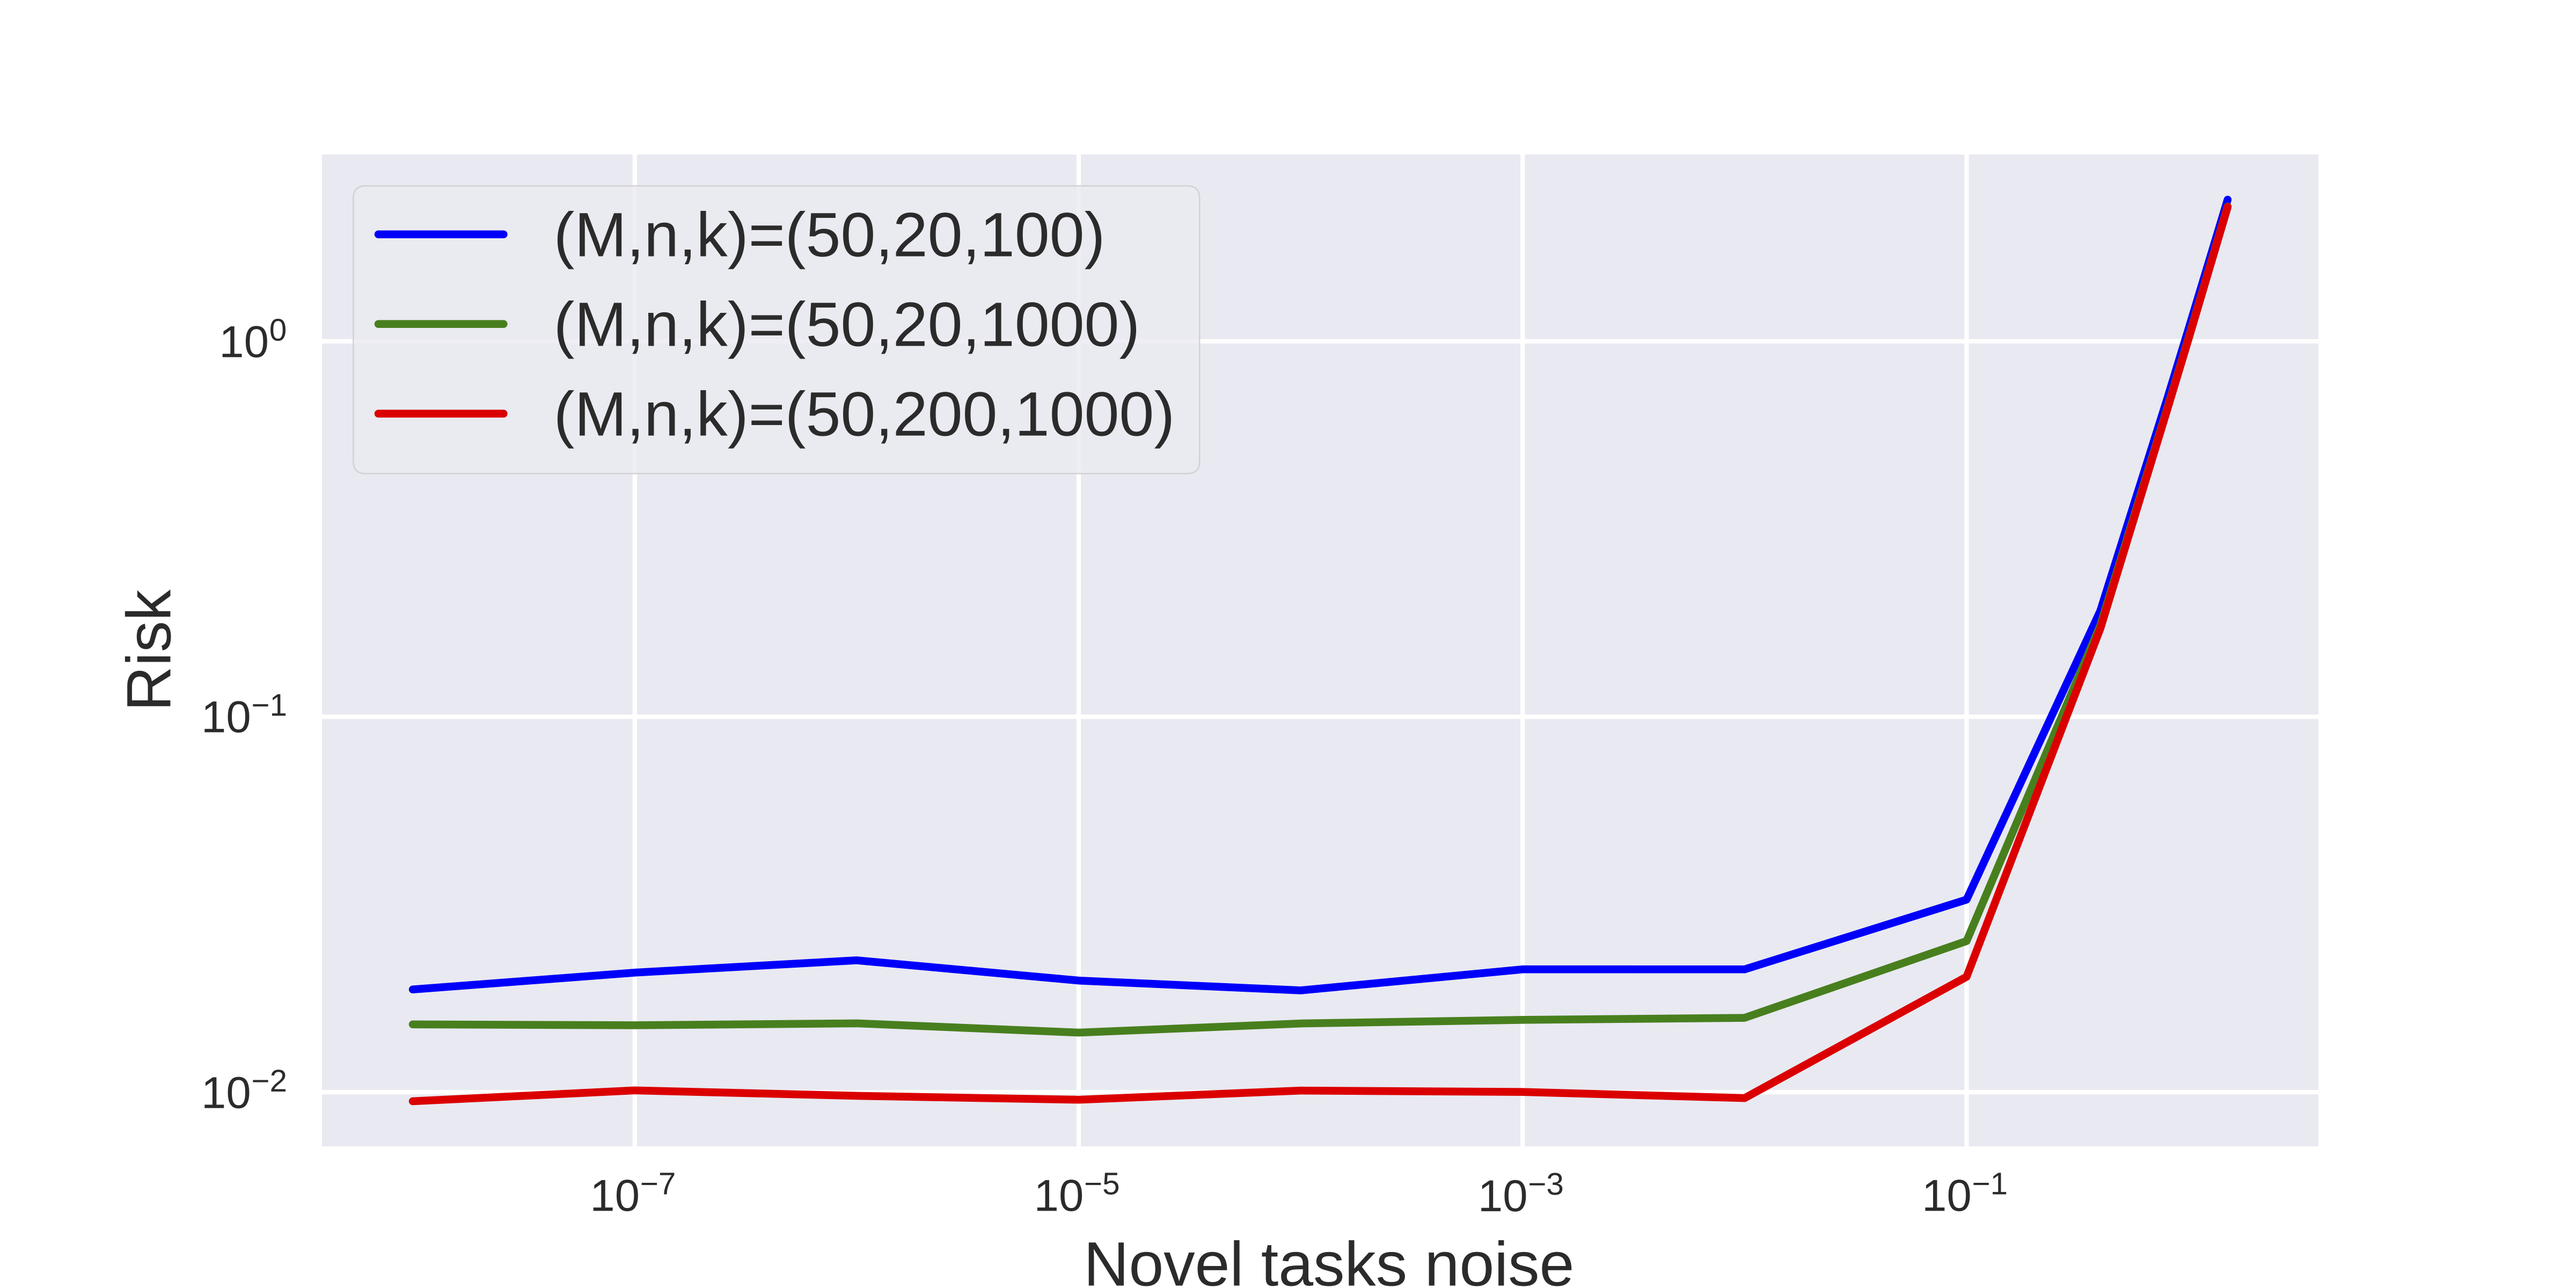
\includegraphics[width=4\linewidth]{main/images/maml_sinusoid.png}
  \caption{Average risk for regressing sinusoid functions with MAML.}
  \label{fig:maml_sinusoid}
\end{figure}
\else
\begin{wrapfigure}{r}{0.48\textwidth}
  \begin{center}
    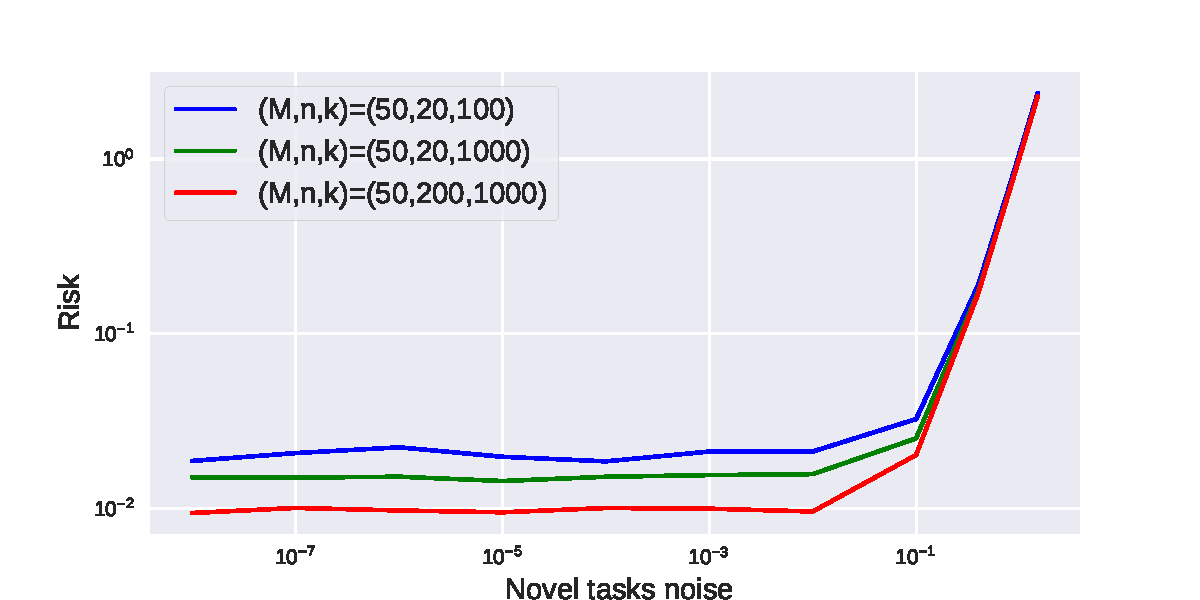
\includegraphics[width=0.48\textwidth]{main/images/maml_sinusoid.pdf}
  \end{center}
  \caption{Average risk for regressing sinusoid functions with MAML.}
  \label{fig:maml_sinusoid}
\end{wrapfigure}
\fi

We display the risk averaged over 30 trials in Figure~\ref{fig:maml_sinusoid}. We varied the novel task difficulty by increasing the observation noise in the novel task.
We plot separate curves for different dataset size configurations, and observe that the empirical results align fairly well with the results derived by sampling the hierarchical model (Figure \ref{fig:hierarchical_lreg_simulation}A). Adding more meta-training data (increasing $n$) is beneficial (green vs. yellow)
and adding more test data-points (higher $k$) is also beneficial (red vs. green).  Here however, these relationships did not interact with the task difficulty, as the wins for increased meta-training and meta-testing data were consistent, until task noise prevents any setting of the model from performing the task.
